%!TeX program = xelatex
\documentclass{coursework}

% Подключение пакетов (float для [H], minted для кода)
\usepackage{float}
\usepackage{csquotes}
\usepackage{minted}
\usepackage{listings}
\usepackage{lipsum}
\usepackage{enumitem}
\usepackage{tabularx}
\usepackage{multirow} % <--- ДОБАВЬТЕ ЭТУ СТРОКУ ДЛЯ ИСПРАВЛЕНИЯ ОШИБКИ Таблицы!

\usepackage{fontspec}
\setmonofont{Courier New} % задаём моноширинный шрифт

\usepackage{listings}
\lstset{
    basicstyle=\ttfamily\footnotesize, % <--- ЗДЕСЬ УВЕЛИЧИЛИ ШРИФТ!
    language=C++,
    keywordstyle=\bfseries, % пример настройки ключевых слов
    numbers=left,           % нумерация строк слева
    numberstyle=\tiny
}

%
%   В цьому окремому файлі визначимо власні команди,
%   щоб не засмічувати головний файл
%


%                        Custom colors
% --------------------------------------------------------------
\definecolor{grey50}{HTML}{FAFAFA}
\definecolor{bluegray400}{HTML}{78909C}

%                      Custom text commands
% --------------------------------------------------------------
\newcommand{\alert}[1]{{\color{red} #1}}
\newcommand{\Alert}[1]{\textbf{\alert{#1}}}

\newcommand{\hl}[1]{\textit{#1}}
\newcommand{\Hl}[1]{\textbf{\textit{#1}}}
\newcommand{\HL}[1]{\textbf{#1}}

\newcommand{\code}[1]{\texttt{#1}}



%                    JS code formatting with minted
% --------------------------------------------------------------
% \newenvironment{longlisting}{\captionsetup{type=listing}}{}

% Define line numbering style
% \renewcommand\theFancyVerbLine{\color{bluegray400} \small \arabic{FancyVerbLine}}

% \js- команда для форматування коду прямо в рядку тексту.
% \NewDocumentCommand{\js}{v}{%
%  \usemintedstyle{friendly}%
%  \mintinline{js}|#1|
%}

% Оточеня jscode для форматоування коду як лістингу
% \newenvironment{jscode}
%    {\VerbatimEnvironment
%    \usemintedstyle{friendly}
%     \begin{minted}[breaklines, obeytabs, tabsize=4, xleftmargin=24pt, linenos, bgcolor=grey50]{js}}
%    {\end{minted}}

% Команда для включення вихідних файлів програм мовою c++
% \newcommand{\inputjs}[1]{%
%     \inputminted[breaklines, tabsize=4, obeytabs, xleftmargin=24pt,linenos]{js}{#1}%
%}  

%                    Rust code formatting with minted
% --------------------------------------------------------------
\newenvironment{longlisting}{\captionsetup{type=listing}}{}

% Define line numbering style
\renewcommand\theFancyVerbLine{\color{bluegray400} \small \arabic{FancyVerbLine}}

% \rs- команда для форматування коду прямо в рядку тексту.
\NewDocumentCommand{\rs}{v}{%
    %\usemintedstyle{friendly}%
    \usemintedstyle{vs}%
    \mintinline{rust}|#1|
}

\newenvironment{cppcode}
{\hrule\vspace{4pt}
    \VerbatimEnvironment%
    %\usemintedstyle{tango}%
    \usemintedstyle{vs}%
    \fontsize{10pt}{12pt}\selectfont%
    \setlength\partopsep{-\topsep}%
    \begin{minted}[breaklines, obeytabs, tabsize=4]{cpp}}
    {\end{minted}\vspace{4pt}\hrule}


% Команда для включення вихідних файлів програм мовою C++
\newcommand{\inputcpp}[1]{{% 🛠️ Добавили открывающую скобку тут
        \usemintedstyle{vs}
        \fontsize{10pt}{12pt}\selectfont
        \inputminted[breaklines, obeytabs, tabsize=2]{cpp}{#1}%
    }} % 🛠️ И закрывающую скобку тут

%                    Java code formatting with minted
% --------------------------------------------------------------

% Команда для автоматического включения файлов Java с мелкими номерами строк и рамками
\newcommand{\inputjava}[1]{{%
    \usemintedstyle{vs} % Используем стиль VS, как в C++
    \fontsize{8pt}{10pt}\selectfont % Размер шрифта самого кода
    
    % Локальное переопределяем размер номеров строк ТОЛЬКО внутри этой команды
    \renewcommand\theFancyVerbLine{\color{bluegray400} \scriptsize \arabic{FancyVerbLine}}%
    
    \inputminted[
        %frame=lines,      % Горизонтальные рамки сверху и снизу
        %framesep=2mm,     % Отступ кода от рамок
        baselinestretch=0.9,
        linenos,          % Включаем нумерацию
        breaklines,       % Перенос длинных строк
        tabsize=4         % Табуляция для Java
    ]{java}{#1}%
}}


% Настройка библиографии Biber
%\usepackage[backend=biber,style=gost-numeric,sorting=none]{biblatex}
%\addbibresource{references.bib}

% Настройки титульного листа
\university{Національний університет \enquote{Одеська політехніка}}
\department{Кафедра інформаційних технологій}

\discipline{\enquote{Об’єктно-орієнтоване та подійно-орієнтоване програмування}}
\title{\enquote{Знайомство з базовим синтаксисом та операторами Java}}
%\variant{7}

\tutor[male]{к т.н., доцент Рудніченко М.Д.}
\author[male]{Горбунова А.А.}
\course{II}
\group{AД-251}
\speciality{F6}
\city{ДУОП}
\year{2026}

\begin{document}

% Элементы титульного листа / Содержания (зависят от реализации класса)
\maketitle		% титульный лист
%\makecontents		% содержание

% Подключение модулей пояснительной записки
\section{Мета роботи та завдання}

\textbf{Мета роботи:}
\begin{enumerate}
    \item Встановити необхідне програмне забезпечення для програмування на ЯП \texttt{Java};
    \item Ознайомитися з базовим синтаксисом мови та основними операторами;
    \item Вивчити приклади угоди щодо коду для ЯП \texttt{Java}.
\end{enumerate}

\skipline
\textbf{Завдання на лабораторну роботу:}
\begin{enumerate}
    \item 
    Напишіть метод, який приймає на вхід масив цілих чисел (довжиною 2 і більше) і 
    повертає true, якщо в масиві кожен елемент більше або дорівнює попередньому. Інакше він повертає false.
    \item 
    Напишіть метод, 
    який виводить на екран числа від 1 до 100. При цьому замість чисел, кратних трьох, 
    програма повинна виводити слово Fizz, а замість чисел, кратних п'яти - слово Buzz. 
    Якщо число кратне і 3, і 5, програма повинна виводити слово «FizzBuzz».
    \item 
    Реалізуйте метод, який приймає на вхід масив цілих чисел (довжиною 2 або більше) і повертає true, 
    якщо масив можна розділити так, щоб сума чисел в обох частинах була рівною і false інакше.
\end{enumerate}

\section{Обґрунтування вибору та налаштування середовища розробки}

\subsection{Аналіз інструментарію та обґрунтування вибору VS Code}

Згідно з методичними вказівками, для розробки програмного забезпечення на мові Java 
традиційно розглядається ``велика трійка'' інтегрованих середовищ розробки (IDE): NetBeans, 
Eclipse та IntelliJ IDEA. Проте в межах виконання даної лабораторної роботи було прийнято 
рішення відмовитися від стандартних автоматизованих майстрів генерації проектів на користь 
легковажного та універсального текстового редактора \textbf{Visual Studio Code (VS Code)}.

Такий підхід має низку суттєвих інженерних та освітніх переваг:
\begin{itemize}
    \item \textbf{Глибоке розуміння процесів компіляції:} 
    Використання автоматизованих систем збирання (Maven, Gradle) на початковому етапі приховує 
    від розробника внутрішні механізми взаємодії компілятора та віртуальної машини. Створення 
    проекту ``з нуля'' дозволяє повністю контролювати структуру каталогів та процес збирання 
    на рівні утиліт CLI.
    \item \textbf{Єдиний робочий простір (All-in-One):} 
    VS Code дозволяє об'єднати розробку вихідного коду мовою Java та верстку технічного 
    звіту (протоколу) в системі комп'ютерного набору \texttt{LaTeX} в межах одного вікна редактора.
    \item \textbf{Ефективність використання ресурсів:} На відміну від важких IDE, VS Code 
    має високу швидкість роботи та низькі вимоги до оперативної пам'яті, забезпечуючи при 
    цьому повноцінну підтримку мовного сервера Java.
\end{itemize}

\subsection{Встановлення програмного забезпечення та конфігурація системи}

Процес розгортання робочого оточення складався з наступних етапів:
\begin{enumerate}
    \item \textbf{Встановлення інструментарію Java:} 
    У систему було встановлено актуальний комплект розробника\\
     \texttt{Java Development Kit версії 27 (JDK-27)},
    який включає компілятор \texttt{javac} та виконавче середовище JVM.
    \item \textbf{Розширення VS Code:} 
    Для забезпечення інтелектуального аналізу коду (IntelliSense) та підсвічування синтаксису 
    в редактор було інтегровано офіційний пакет розширень \textit{Extension Pack for Java} від Microsoft.
    \item \textbf{Налаштування локалізації терміналу:} Для коректного відображення унікальних літер 
    українського алфавіту \textit{і}, \textit{ї}, \textit{є} у консолі Windows, сесію оболонки 
    було програмно переведено на роботу зі стандартом кодування \texttt{UTF-8}.
\end{enumerate}

\subsection{Автоматизація збирання та формування єдиного циклу розробки}

Для повної автоматизації рутинних операцій компіляції коду та генерації звіту було створено 
кастомний сценарій планувальника завдань всередині файлу \texttt{.vscode/tasks.json}. Облочкою виконання 
було обрано середовище Windows PowerShell.

Розроблена конфігурація об'єднує два послідовних процеси (Завдання) в один ультимативний цикл збирання:
\begin{enumerate}
    \item \textbf{Завдання компіляції та запуску Java:} 
    Компілює всі вихідні файли пакету за допомогою \texttt{javac} із примусовим прапорцем \texttt{-encoding UTF-8}, 
    зберігає бінарні файли \texttt{.class} у каталог \texttt{bin}, ініціалізує UTF-8 кодування консолі та запускає 
    віртуальну машину \texttt{java.exe} для виконання класу \texttt{Main}.
    \item \textbf{Завдання верстки звіту:} Переходить у каталог \texttt{report} та викликає компілятор \texttt{xelatex} 
    із прапорцем \texttt{-shell-escape} для генерації підсумкового PDF-документа, автоматично підтягуючи оновлені 
    лістинги коду.
\end{enumerate}

Завдяки такій конфігурації, натисканням однієї комбінації клавіш \texttt{Ctrl + Shift + B} виконується повний цикл: 
від перевірки працездатності алгоритмів Java до формування фінального друкованого протоколу лабораторної роботи.

\subsection{Реалізація концепції базового пакету та структури проєкту вручну}

Згідно з методичними вказівками, під час створення проєкту в IntelliJ IDEA особлива увага приділяється налаштуванню 
параметра \textbf{Base package} (базового пакету) у форматі \texttt{[назва\_групи].[прізвище]} (наприклад, \texttt{ad251.gorbunova})~\cite{1}. 
У мові Java концепція пакетів (\texttt{package}) виконує роль просторів імен і логічного групування класів, але її 
фундаментальною особливістю є те, що \textbf{структура пакетів в коді повинна строго відповідати фізичній структурі папок на диску}.

Під час кастомного налаштування проєкту у VS Code цей процес не приховувався за автоматичними майстрами IDE, 
а був реалізований повністю вручну за такими етапами:

\begin{enumerate}
    \item \textbf{Створення фізичної ієрархії каталогів:} 
    У корені робочого простору було створено каталог вихідного коду \texttt{src}, всередині якого вручную розгорнуто 
    ланцюжок папок, що точно відповідає структурі базового пакету: \texttt{src/ad251/gorbunova/}.
    \item \textbf{Конфігурація логічного кореня (Source Root):} 
    Для того щоб мовний сервер Java у VS Code коректно інтерпретував ієрархію, у файлі налаштувань 
    середовища \texttt{.vscode/settings.json} було явно вказано шлях до вихідних файлів за допомогою параметра:
    \begin{verbatim}
    "java.project.sourcePaths": ["src"]
    \end{verbatim}
    Завдяки цьому середовище починає відлік простору імен саме з папки \texttt{src}, 
    і шлях \texttt{src/ad251/gorbunova/Main.java} стає повністю еквівалентним 
    оголошенню \texttt{package ad251.gorbunova;} в першому рядку кожного файлу.
    \item \textbf{Ізоляція артефактів збирання:} 
    На відміну від стандартного підходу, де скомпільовані файли суміщаються з вихідним кодом, за допомогою 
    прапорця \texttt{-d bin} утиліти \texttt{javac} було налаштовано автоматичне дзеркальне створення структури 
    пакетів у відокремленому бінарному каталозі \texttt{bin/ad251/gorbunova/}.
\end{enumerate}

На рисунку~\ref{fig:project_tree} представлено фінальну архітектуру та дерево папок розробленого 
проєкту, згенероване безпосередньо в робочому просторі.

\begin{figure}[H]
    \centering
    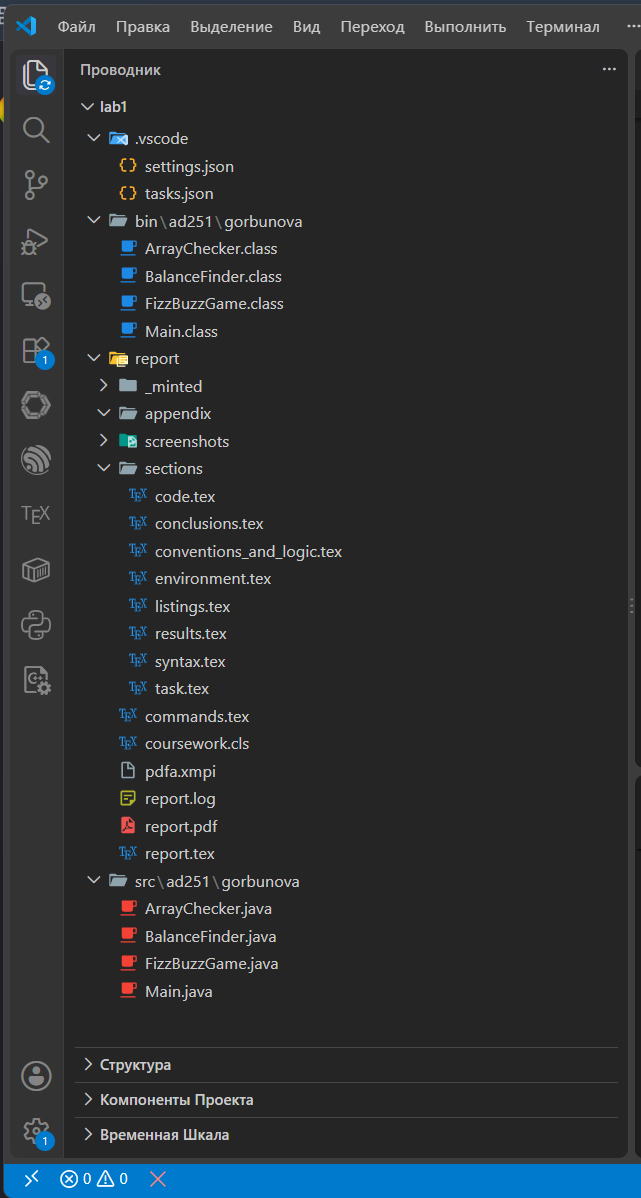
\includegraphics[width=0.45\textwidth]{screenshots/project_tree.png}
    \caption{Фізична структура каталогів проєкту із реалізацією базового пакету \texttt{ad251.gorbunova}}
    \label{fig:project_tree}
\end{figure}



\section{Аналіз базового синтаксису та операторів: порівняльний аспект із C/C++}

\subsection{Загальні синтаксичні конструкції та типи даних}

Оскільки синтаксис мови Java історично базується на мовах C та C++, базові керуючі 
конструкції (цикли \texttt{for}, \texttt{while}, \texttt{do-while} та оператори 
розгалуження \texttt{if-else}, \texttt{switch}) є практично ідентичними. Проте на 
рівні базової архітектури та типізації мови мають суттєві відмінності:

\begin{itemize}
    \item \textbf{Строга типізація та незалежність від платформи:} 
    На відміну від C/C++,  де розмір типу \texttt{int} чи \texttt{long} залежить 
    від архітектури процесора та компілятора, у Java всі примітивні типи мають фіксований 
    розмір у пам'яті на будь-якій платформі (наприклад, \texttt{int} завжди 32 біти, \texttt{long} — 64 біти).
    \item \textbf{Відсутність беззнакових типів:} 
    У Java відсутній модифікатор \texttt{unsigned}. Усі числові примітивні 
    типи (включаючи \texttt{byte} та \texttt{short}) є виключно знаковими.
    \item \textbf{Булевий тип даних:} 
    На відміну від C, де логічна умова може оперувати цілими числами (де \texttt{0} — це \texttt{false}, 
    а будь-яке інше число — \texttt{true}), у Java тип \texttt{boolean} є ізольованим. Конструкції 
    розгалуження приймають виключно значення \texttt{true} або \texttt{false}, що унеможливлює помилки 
    вигляду \texttt{if (a = b)}.
\end{itemize}

\subsection{Ключові відмінності в роботі з пам'яттю та об'єктами}

В межах виконання лабораторної роботи було досліджено три фундаментальні відмінності Java від мов C/C++, 
які критично впливають на проектування програм:

\begin{enumerate}
    \item \textbf{Повна відсутність вказівників:} 
    У Java повністю вилучено арифметику вказівників, прямий доступ до адрес пам'яті та 
    оператори \texttt{*}, \texttt{\&}, \texttt{->}. Усі об'єкти та масиви є посилальними 
    типами й керуються через безпечні посилання.
    \item \textbf{Автоматичне керування пам'яттю (Garbage Collection):} 
    Розробнику більше не потрібно вручну звільняти пам'ять за допомогою \texttt{free()} 
    чи \texttt{delete}. Об'єкти створюються у кучі (\texttt{heap}) за допомогою ключового 
    слова \texttt{new}, а збірник сміття (GC) автоматично утилізує їх, коли на них не залишається 
    активних посилань.
    \item \textbf{Масиви як повноцінні об'єкти:} 
    На відміну від C/C++, де масив є просто вказівником на перший елемент і вимагає окремої
     передачі його розміру у функції, в Java масив є об'єктом. Він інкапсулює у собі 
     властивість \texttt{length}, що дозволяє безпечно контролювати межі ітерацій і унеможливлює 
     помилку переповнення буфера (\texttt{ArrayIndexOutOfBoundsException}).
\end{enumerate}

\section{Стандарти оформлення коду та архітектура алгоритмів}

\subsection{Дотримання конвенції Oracle Code Conventions}

У межах виконання лабораторної роботи особливу увагу було приділено стандартам 
інженерного оформлення вихідного коду згідно з вимогами \textit{Oracle Code Conventions}. 
Було опановано та застосовано на практиці такі правила:

\begin{itemize}
    \item \textbf{Угода про іменування (Naming Conventions):} 
    Імена всіх створених компонентів та класів (\texttt{ArrayChecker}, \texttt{FizzBuzzGame}, \texttt{BalanceFinder}) 
    записані у стилі \texttt{UpperCamelCase}. Назви методів та змінних (\texttt{isSortedUp()}, \texttt{totalSum}, \texttt{leftSum}) 
    строго відповідають стилю \texttt{lowerCamelCase}, де перше слово обов'язково є дієсловом для методів та іменником для змінних.
    \item \textbf{Стандартизація коментарів:} Структура кожного файлу містить три рівні документування:
    \begin{enumerate}
        \item \textit{Блок Copyright} у самому верху файлу із зазначенням ліцензії Apache 2.0 та автора.
        \item \textit{JavaDoc коментарі} (\texttt{/** ... */}) перед класами та методами із 
        застосуванням тегів \texttt{@author}, \texttt{@version}, \texttt{@param} та \texttt{@return}.
        \item \textit{Внутрішні коментарі} (\texttt{/* ... */} та \texttt{//}) для 
        пояснення складних ділянок бізнес-логіки з обов'язковим відступом у один порожній рядок перед ними.
    \end{enumerate}
\end{itemize}

\section{Структура проекту, логіка завдань та вихідний код програми}

На відміну від процедурного підходу, кожне завдання лабораторної роботи було інкапсульовано 
в окремий автономний клас-компонент, що дозволило уникнути використання статичних методів у стилі мови C.

\begin{enumerate}
    \item \textbf{Перевірка впорядкованості масиву (Клас \texttt{ArrayChecker}):} 
    \\Алгоритм виконує один лінійний прохід по масиву починаючи з індексу \texttt{1}. 
    Якщо поточний елемент виявляється меншим за попередній, метод негайно повертає \texttt{false}, 
    що оптимізує швидкість виконання.
    \item \textbf{Матричне виведення FizzBuzz (Клас \texttt{FizzBuzzGame}):} 
    \\Для створення компактного та зручного для звітності інтерфейсу, логіку перевірки 
    відповідно до заданої кратності чисел (на 3, 5 та їхній добуток) було об'єднано з 
    формативаним виведенням \texttt{System.out.printf("\%-10s")}. Це дозволило згенерувати 
    результати у вигляді математичної сітки розміром 10 на 10 стовпців.
    \item \textbf{Пошук балансу сум (Клас \texttt{BalanceFinder}):} 
    \\Спочатку обчислюється повна сума 
    масиву, а під час другого лінійного проходу накопичується ліва частина. Рівновагу 
    знайдено в момент, коли ліва сума стає рівною рівно половині загальної суми.
    \item \textbf{Координація та точка входу (Клас \texttt{Main}):} 
    \\Клас містить обов'язковий для виконання Java-додатків метод \texttt{public static void main(String[] args)}. 
    Назначенням цього компонента є повне управління життєвим циклом програми ініціалізує тестові масиви даних, 
    виконує обчислення та створює екземпляри класів \texttt{ArrayChecker}, \texttt{FizzBuzzGame} \\
    та \texttt{BalanceFinder}, передає їм аргументи через конструктори та виводить фінальні результати обчислень у термінал середовища розробки.
\end{enumerate}


\section{Лістинг програмного коду}

У цьому розділі наведено повний вихідний код розробленої структури класів. 
Код оформлено згідно зі стандартами \textit{Oracle Code Conventions} та містить 
вичерпну документацію у форматі \textit{JavaDoc}.

\subsection{Клас Main.java}
\inputjava{../src/ad251/gorbunova/Main.java}

\newpage % <- Перенос следующего листинга на новую страницу
\subsection{Клас ArrayChecker.java}
\inputjava{../src/ad251/gorbunova/ArrayChecker.java}

\newpage % <- Перенос следующего листинга на новую страницу
\subsection{Клас FizzBuzzGame.java}
\inputjava{../src/ad251/gorbunova/FizzBuzzGame.java}

\newpage % <- Перенос следующего листинга на новую страницу
\subsection{Клас BalanceFinder.java}
\inputjava{../src/ad251/gorbunova/BalanceFinder.java}



\section{Результати роботи програми}

Для верифікації правильності роботи розроблених алгоритмів було здійснено запуск програми в 
єдиному циклі збирання середовища VS Code. На рисунку~\ref{fig:terminal} представлено фінальне 
виведення результатів у термінал Windows PowerShell.

\begin{figure}[H]
    \centering
    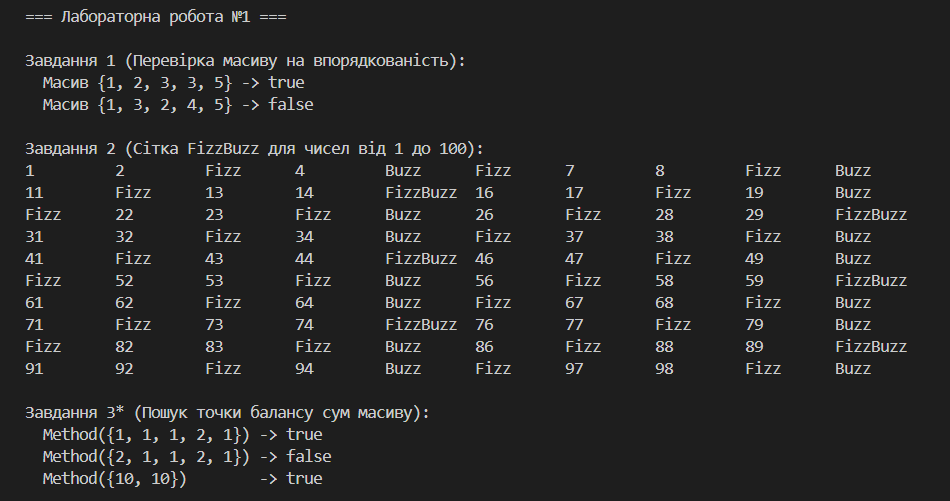
\includegraphics[width=0.95\textwidth]{screenshots/terminal_output.png}
    \caption{Вигляд терміналу після успішного виконання всіх трьох завдань лабораторної роботи}
    \label{fig:terminal}
\end{figure}

Як видно з результатів тестування:
\begin{itemize}
    \item 
    Компонент \texttt{ArrayChecker} коректно визначив впорядкованість першого 
    масиву (\texttt{true}) та зафіксував порушення порядку у другому (\texttt{false}).
    \item 
    Гра \texttt{FizzBuzzGame} згенерувала компактну текстову матрицю 
    розміром $10 \times 10$ елементів із правильним заміщенням чисел на відповідні мовні маркери.
    \item 
    Оптимізований обчислювач \texttt{BalanceFinder} безпомилково знайшов точки 
    рівноваги сум для демонстраційних масивів.
\end{itemize}

\section{Висновки:}

В ході виконання лабораторної роботи було успішно досягнуто поставлену мету: 
розгорнуто кастомне робоче оточення для програмування на мові Java та опановано 
базовий синтаксис і оператори цієї мови через призму порівняльного аналізу з екосистемою C/C++.

На основі виконаних досліджень та розробленого програмного комплексу сформульовано такі науково-практичні висновки:
\begin{enumerate}
    \item \textbf{Ефективність інструментарію:} 
    Ручне налаштування універсального редактора VS Code та інтеграція компілятора JDK-27 
    за допомогою сценаріїв автоматизації Windows PowerShell (\texttt{tasks.json}) дозволили 
    створити прозорий та ефективний цикл збирання проєкту «з нуля». Такий підхід забезпечив 
    повний контроль над структурою пакетів та процесом компіляції без використання ваговитих 
    сторонніх систем збирання.
    \item \textbf{Концептуальні переваги Java:} 
    Практична реалізація алгоритмів підтвердила ключові архітектурні відмінності Java від 
    мов C/C++. Відсутність ручного керування пам'яттю та вказівників (завдяки роботі Garbage Collector), 
    строга ізоляція булевого типу та робота з масивами як з повноцінними об'єктами (властивість \texttt{length}) 
    суттєво підвищують безпеку розробки та нівелюють ризики виникнення критичних помилок переповнення буфера.
    \item \textbf{Об'єктно-орієнтована декомпозиція:} 
    На відміну від процедурного стилю, завдання лабораторної роботи були успішно розділені на ізольовані 
    класи-компоненти (\texttt{ArrayChecker}, \texttt{FizzBuzzGame}, \texttt{BalanceFinder}) із чіткою 
    інкапсуляцією логіки, що заклало правильний фундамент для подальшого вивчення об'єктно-орієнтованого програмування.
    \item \textbf{Культура розробки:} 
    Весь вихідний код програми був повністю адаптований до суворих вимог міжнародного стандарту \textit{Oracle Code Conventions}. 
    Впровадження трирівневої системи коментування (ліцензійний блок, JavaDoc-документація та внутрішні пояснення) разом із 
    автоматичною збіркою звіту в системі \texttt{LaTeX} дозволили вивести фінальну технічну документацію на рівень промислових стандартів розробки.
\end{enumerate}


\newpage
\section{Інформаційні ресурси та посилання на вихідний код}

Згідно з вимогами до здачі лабораторної роботи, повний проєкт вихідного коду розробленого 
додатку розміщено у віддаленому репозиторії системи контролю версій. 

\begin{itemize}
    \item \textbf{Посилання на Git-репозиторій проєкту:} \\
    \url{https://github.com/nasuehfw/oop-lab1.git}
    
    \item \textbf{Електронний каталог спільного доступу:} \\
    \url{https://drive.google.com/drive/folders/1mIulRQSfoHAyQ2GnqdQbwGz2dFX-5VGK?usp=drive\_link}
\end{itemize}

%\input{sections/summary.tex}
%\input{sections/questions.tex}


%\input{sections/3_network_resources_and_accesstesting.tex}
%\input{sections/4_deployment_practice.tex}

% Выводы
%\input{sections/summary.tex}

% Литератупа
%\makebibliography
%\input{sections/literature.tex}

% Аппендикс (если нужен)
%\appendix
%\input{appendix/appendix.tex}


\end{document}
